\documentclass[twoside]{book}

% Packages required by doxygen
\usepackage{fixltx2e}
\usepackage{calc}
\usepackage{doxygen}
\usepackage{graphicx}
\usepackage[utf8]{inputenc}
\usepackage{makeidx}
\usepackage{multicol}
\usepackage{multirow}
\PassOptionsToPackage{warn}{textcomp}
\usepackage{textcomp}
\usepackage[nointegrals]{wasysym}
\usepackage[table]{xcolor}

% Font selection
\usepackage[T1]{fontenc}
\usepackage{mathptmx}
\usepackage[scaled=.90]{helvet}
\usepackage{courier}
\usepackage{amssymb}
\usepackage{sectsty}
\renewcommand{\familydefault}{\sfdefault}
\allsectionsfont{%
  \fontseries{bc}\selectfont%
  \color{darkgray}%
}
\renewcommand{\DoxyLabelFont}{%
  \fontseries{bc}\selectfont%
  \color{darkgray}%
}
\newcommand{\+}{\discretionary{\mbox{\scriptsize$\hookleftarrow$}}{}{}}

% Page & text layout
\usepackage{geometry}
\geometry{%
  a4paper,%
  top=2.5cm,%
  bottom=2.5cm,%
  left=2.5cm,%
  right=2.5cm%
}
\tolerance=750
\hfuzz=15pt
\hbadness=750
\setlength{\emergencystretch}{15pt}
\setlength{\parindent}{0cm}
\setlength{\parskip}{0.2cm}
\makeatletter
\renewcommand{\paragraph}{%
  \@startsection{paragraph}{4}{0ex}{-1.0ex}{1.0ex}{%
    \normalfont\normalsize\bfseries\SS@parafont%
  }%
}
\renewcommand{\subparagraph}{%
  \@startsection{subparagraph}{5}{0ex}{-1.0ex}{1.0ex}{%
    \normalfont\normalsize\bfseries\SS@subparafont%
  }%
}
\makeatother

% Headers & footers
\usepackage{fancyhdr}
\pagestyle{fancyplain}
\fancyhead[LE]{\fancyplain{}{\bfseries\thepage}}
\fancyhead[CE]{\fancyplain{}{}}
\fancyhead[RE]{\fancyplain{}{\bfseries\leftmark}}
\fancyhead[LO]{\fancyplain{}{\bfseries\rightmark}}
\fancyhead[CO]{\fancyplain{}{}}
\fancyhead[RO]{\fancyplain{}{\bfseries\thepage}}
\fancyfoot[LE]{\fancyplain{}{}}
\fancyfoot[CE]{\fancyplain{}{}}
\fancyfoot[RE]{\fancyplain{}{\bfseries\scriptsize Generated on Fri Mar 9 2018 14\+:27\+:59 for My Project by Doxygen }}
\fancyfoot[LO]{\fancyplain{}{\bfseries\scriptsize Generated on Fri Mar 9 2018 14\+:27\+:59 for My Project by Doxygen }}
\fancyfoot[CO]{\fancyplain{}{}}
\fancyfoot[RO]{\fancyplain{}{}}
\renewcommand{\footrulewidth}{0.4pt}
\renewcommand{\chaptermark}[1]{%
  \markboth{#1}{}%
}
\renewcommand{\sectionmark}[1]{%
  \markright{\thesection\ #1}%
}

% Indices & bibliography
\usepackage{natbib}
\usepackage[titles]{tocloft}
\setcounter{tocdepth}{3}
\setcounter{secnumdepth}{5}
\makeindex

% Hyperlinks (required, but should be loaded last)
\usepackage{ifpdf}
\ifpdf
  \usepackage[pdftex,pagebackref=true]{hyperref}
\else
  \usepackage[ps2pdf,pagebackref=true]{hyperref}
\fi
\hypersetup{%
  colorlinks=true,%
  linkcolor=blue,%
  citecolor=blue,%
  unicode%
}

% Custom commands
\newcommand{\clearemptydoublepage}{%
  \newpage{\pagestyle{empty}\cleardoublepage}%
}


%===== C O N T E N T S =====

\begin{document}

% Titlepage & ToC
\hypersetup{pageanchor=false,
             bookmarks=true,
             bookmarksnumbered=true,
             pdfencoding=unicode
            }
\pagenumbering{roman}
\begin{titlepage}
\vspace*{7cm}
\begin{center}%
{\Large My Project }\\
\vspace*{1cm}
{\large Generated by Doxygen 1.8.7}\\
\vspace*{0.5cm}
{\small Fri Mar 9 2018 14:27:59}\\
\end{center}
\end{titlepage}
\clearemptydoublepage
\tableofcontents
\clearemptydoublepage
\pagenumbering{arabic}
\hypersetup{pageanchor=true}

%--- Begin generated contents ---
\chapter{Class Index}
\section{Class List}
Here are the classes, structs, unions and interfaces with brief descriptions\+:\begin{DoxyCompactList}
\item\contentsline{section}{\hyperlink{structmarket__rates__struct}{market\+\_\+rates\+\_\+struct} \\*Estructura de memoria compartida de cotizaciones }{\pageref{structmarket__rates__struct}}{}
\item\contentsline{section}{\hyperlink{structmsgbuf}{msgbuf} \\*Estructura de colas de mensajes }{\pageref{structmsgbuf}}{}
\item\contentsline{section}{\hyperlink{structrace__control__struct}{race\+\_\+control\+\_\+struct} \\*Estructura de memoria compartida de control de carrera }{\pageref{structrace__control__struct}}{}
\end{DoxyCompactList}

\chapter{File Index}
\section{File List}
Here is a list of all documented files with brief descriptions\+:\begin{DoxyCompactList}
\item\contentsline{section}{\hyperlink{ejercicio2_8c}{ejercicio2.\+c} \\*Ejercicio2 Creación de 4 procesos hijos que duermen durante 30s mientras que el proceso padre espera 5s y después envía a cada proceso hijo la señal de finalización S\+I\+G\+T\+E\+RM }{\pageref{ejercicio2_8c}}{}
\item\contentsline{section}{\hyperlink{ejercicio4_8c}{ejercicio4.\+c} \\*Ejercicio4 Manejo de señales entre procesos hijos y padre }{\pageref{ejercicio4_8c}}{}
\item\contentsline{section}{\hyperlink{ejercicio6a_8c}{ejercicio6a.\+c} \\*Ejercicio6a Toma de contacto con la funcion alarm() }{\pageref{ejercicio6a_8c}}{}
\item\contentsline{section}{\hyperlink{ejercicio6b_8c}{ejercicio6b.\+c} \\*Ejercicio6b Toma de contacto con la funcion sigfillset() }{\pageref{ejercicio6b_8c}}{}
\item\contentsline{section}{\hyperlink{semaforos_8c}{semaforos.\+c} \\*Ejercicio9 }{\pageref{semaforos_8c}}{}
\item\contentsline{section}{\hyperlink{semaforos_8h}{semaforos.\+h} \\*Utilidades de manejo de semaforos }{\pageref{semaforos_8h}}{}
\end{DoxyCompactList}

\chapter{Class Documentation}
\hypertarget{structArgum}{\section{Argum Struct Reference}
\label{structArgum}\index{Argum@{Argum}}
}


Estructura de argumentos de entrada.  


\subsection*{Public Attributes}
\begin{DoxyCompactItemize}
\item 
int \hyperlink{structArgum_a1e19639236d672db337655913280c502}{id}
\item 
int $\ast$$\ast$ \hyperlink{structArgum_a5e62bf7d3af611b48cdeed5decdf47be}{matrix}
\item 
int \hyperlink{structArgum_a69c560b91efcd6709b891e9a7fd204bd}{dim}
\item 
int \hyperlink{structArgum_a8f60de19f057d334f365ec7ef21d7439}{scalar}
\item 
char $\ast$ \hyperlink{structArgum_a6ba39122df5e87923c854fdb415b37af}{pos1}
\item 
char $\ast$ \hyperlink{structArgum_a69aaf9b57d62f8704a7f83afaca5d361}{pos2}
\end{DoxyCompactItemize}


\subsection{Detailed Description}
Estructura de argumentos de entrada. 

La mision de esta entructura es pasarle todos los argumentos de entrada que necesitan los hilos para su ejecucion 

\subsection{Member Data Documentation}
\hypertarget{structArgum_a69c560b91efcd6709b891e9a7fd204bd}{\index{Argum@{Argum}!dim@{dim}}
\index{dim@{dim}!Argum@{Argum}}
\subsubsection[{dim}]{\setlength{\rightskip}{0pt plus 5cm}int Argum\+::dim}}\label{structArgum_a69c560b91efcd6709b891e9a7fd204bd}
dimension de la matriz \hypertarget{structArgum_a1e19639236d672db337655913280c502}{\index{Argum@{Argum}!id@{id}}
\index{id@{id}!Argum@{Argum}}
\subsubsection[{id}]{\setlength{\rightskip}{0pt plus 5cm}int Argum\+::id}}\label{structArgum_a1e19639236d672db337655913280c502}
Id del hilo \hypertarget{structArgum_a5e62bf7d3af611b48cdeed5decdf47be}{\index{Argum@{Argum}!matrix@{matrix}}
\index{matrix@{matrix}!Argum@{Argum}}
\subsubsection[{matrix}]{\setlength{\rightskip}{0pt plus 5cm}int$\ast$$\ast$ Argum\+::matrix}}\label{structArgum_a5e62bf7d3af611b48cdeed5decdf47be}
matriz de enteros \hypertarget{structArgum_a6ba39122df5e87923c854fdb415b37af}{\index{Argum@{Argum}!pos1@{pos1}}
\index{pos1@{pos1}!Argum@{Argum}}
\subsubsection[{pos1}]{\setlength{\rightskip}{0pt plus 5cm}char$\ast$ Argum\+::pos1}}\label{structArgum_a6ba39122df5e87923c854fdb415b37af}
variable donde hilo1 lee e hilo2 escribe \hypertarget{structArgum_a69aaf9b57d62f8704a7f83afaca5d361}{\index{Argum@{Argum}!pos2@{pos2}}
\index{pos2@{pos2}!Argum@{Argum}}
\subsubsection[{pos2}]{\setlength{\rightskip}{0pt plus 5cm}char$\ast$ Argum\+::pos2}}\label{structArgum_a69aaf9b57d62f8704a7f83afaca5d361}
variable donde hilo1 escribe e hilo2 lee \hypertarget{structArgum_a8f60de19f057d334f365ec7ef21d7439}{\index{Argum@{Argum}!scalar@{scalar}}
\index{scalar@{scalar}!Argum@{Argum}}
\subsubsection[{scalar}]{\setlength{\rightskip}{0pt plus 5cm}int Argum\+::scalar}}\label{structArgum_a8f60de19f057d334f365ec7ef21d7439}
escalar que multiplica la matriz 

The documentation for this struct was generated from the following file\+:\begin{DoxyCompactItemize}
\item 
\hyperlink{ejercicio13_8c}{ejercicio13.\+c}\end{DoxyCompactItemize}

\hypertarget{structStructure}{\section{Structure Struct Reference}
\label{structStructure}\index{Structure@{Structure}}
}


Estructura programa.  


\subsection*{Public Attributes}
\begin{DoxyCompactItemize}
\item 
char \hyperlink{structStructure_a2ab802cb05c7e48647ff1cca1bcfd585}{str} \mbox{[}\hyperlink{ejercicio9_8c_a05b49c662c073f89e86804f7856622a0}{L\+E\+N}\mbox{]}
\item 
int \hyperlink{structStructure_ae554951bcd1248a08201a48ce50b81c4}{n}
\end{DoxyCompactItemize}


\subsection{Detailed Description}
Estructura programa. 

Esta estructura contiene una cadena de caracteres y un entero. 

\subsection{Member Data Documentation}
\hypertarget{structStructure_ae554951bcd1248a08201a48ce50b81c4}{\index{Structure@{Structure}!n@{n}}
\index{n@{n}!Structure@{Structure}}
\subsubsection[{n}]{\setlength{\rightskip}{0pt plus 5cm}int Structure\+::n}}\label{structStructure_ae554951bcd1248a08201a48ce50b81c4}
numero entero \hypertarget{structStructure_a2ab802cb05c7e48647ff1cca1bcfd585}{\index{Structure@{Structure}!str@{str}}
\index{str@{str}!Structure@{Structure}}
\subsubsection[{str}]{\setlength{\rightskip}{0pt plus 5cm}char Structure\+::str}}\label{structStructure_a2ab802cb05c7e48647ff1cca1bcfd585}
cadena de caracteres 

The documentation for this struct was generated from the following files\+:\begin{DoxyCompactItemize}
\item 
\hyperlink{ejercicio12a_8c}{ejercicio12a.\+c}\item 
\hyperlink{ejercicio12b_8c}{ejercicio12b.\+c}\item 
\hyperlink{ejercicio6_8c}{ejercicio6.\+c}\end{DoxyCompactItemize}

\chapter{File Documentation}
\hypertarget{ejercicio12a_8c}{\section{ejercicio12a.\+c File Reference}
\label{ejercicio12a_8c}\index{ejercicio12a.\+c@{ejercicio12a.\+c}}
}


Ejercicio12a Creacion de 100 procesos y en cada uno se calculan los primeros N numeros primos, siendo N pasado como argumento entrada al programa.  


{\ttfamily \#include $<$stdio.\+h$>$}\\*
{\ttfamily \#include $<$stdlib.\+h$>$}\\*
{\ttfamily \#include $<$string.\+h$>$}\\*
{\ttfamily \#include $<$sys/types.\+h$>$}\\*
{\ttfamily \#include $<$sys/wait.\+h$>$}\\*
{\ttfamily \#include $<$unistd.\+h$>$}\\*
{\ttfamily \#include $<$errno.\+h$>$}\\*
{\ttfamily \#include $<$pthread.\+h$>$}\\*
{\ttfamily \#include $<$limits.\+h$>$}\\*
{\ttfamily \#include $<$time.\+h$>$}\\*
{\ttfamily \#include $<$math.\+h$>$}\\*
Include dependency graph for ejercicio12a.\+c\+:
\nopagebreak
\begin{figure}[H]
\begin{center}
\leavevmode
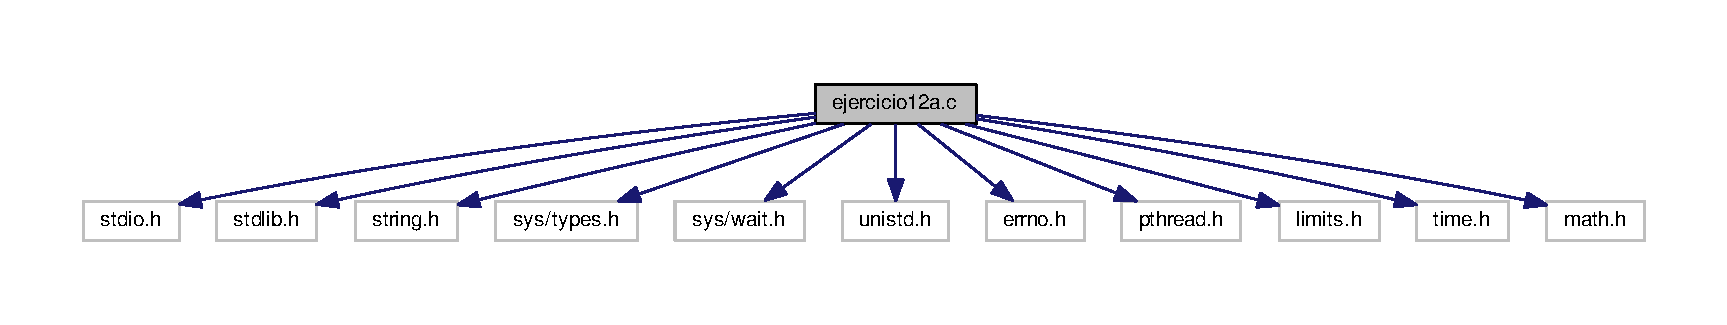
\includegraphics[width=350pt]{ejercicio12a_8c__incl}
\end{center}
\end{figure}
\subsection*{Classes}
\begin{DoxyCompactItemize}
\item 
struct \hyperlink{structStructure}{Structure}
\begin{DoxyCompactList}\small\item\em Estructura programa. \end{DoxyCompactList}\end{DoxyCompactItemize}
\subsection*{Macros}
\begin{DoxyCompactItemize}
\item 
\#define \hyperlink{ejercicio12a_8c_a05b49c662c073f89e86804f7856622a0}{L\+E\+N}~100
\item 
\#define \hyperlink{ejercicio12a_8c_a1dc0370947cd4d4485a36ad37de15139}{T\+E\+N\+T\+O\+T\+H\+E\+N\+I\+N\+E}~1000000000
\item 
\#define \hyperlink{ejercicio12a_8c_a469b1ab8d3ecbd62178c442e0d19c200}{N\+\_\+\+C\+H\+I\+L\+D\+S}~100
\end{DoxyCompactItemize}
\subsection*{Functions}
\begin{DoxyCompactItemize}
\item 
int \hyperlink{ejercicio12a_8c_ad6740255386952216cb75d813243a3ea}{is\+\_\+prime} (int n)
\begin{DoxyCompactList}\small\item\em evalua si un numero es primo o no. \end{DoxyCompactList}\item 
int $\ast$ \hyperlink{ejercicio12a_8c_aca3b2affe916a5464b035bde74fd4fae}{calculate\+\_\+primes} (int n\+\_\+primes)
\begin{DoxyCompactList}\small\item\em devuelve un array con los n\+\_\+primes primeros primos \end{DoxyCompactList}\item 
\hypertarget{ejercicio12a_8c_abf9e6b7e6f15df4b525a2e7705ba3089}{int {\bfseries main} (int argc, char const $\ast$argv\mbox{[}$\,$\mbox{]})}\label{ejercicio12a_8c_abf9e6b7e6f15df4b525a2e7705ba3089}

\end{DoxyCompactItemize}


\subsection{Detailed Description}
Ejercicio12a Creacion de 100 procesos y en cada uno se calculan los primeros N numeros primos, siendo N pasado como argumento entrada al programa. 

\begin{DoxyAuthor}{Author}
Alejandro Santorum \& David Cabornero 
\end{DoxyAuthor}
\begin{DoxyVersion}{Version}
1.\+0 
\end{DoxyVersion}
\begin{DoxyDate}{Date}
02-\/03-\/2018 
\end{DoxyDate}


\subsection{Macro Definition Documentation}
\hypertarget{ejercicio12a_8c_a05b49c662c073f89e86804f7856622a0}{\index{ejercicio12a.\+c@{ejercicio12a.\+c}!L\+E\+N@{L\+E\+N}}
\index{L\+E\+N@{L\+E\+N}!ejercicio12a.\+c@{ejercicio12a.\+c}}
\subsubsection[{L\+E\+N}]{\setlength{\rightskip}{0pt plus 5cm}\#define L\+E\+N~100}}\label{ejercicio12a_8c_a05b49c662c073f89e86804f7856622a0}
Longitud de las cadenas de caracteres \hypertarget{ejercicio12a_8c_a469b1ab8d3ecbd62178c442e0d19c200}{\index{ejercicio12a.\+c@{ejercicio12a.\+c}!N\+\_\+\+C\+H\+I\+L\+D\+S@{N\+\_\+\+C\+H\+I\+L\+D\+S}}
\index{N\+\_\+\+C\+H\+I\+L\+D\+S@{N\+\_\+\+C\+H\+I\+L\+D\+S}!ejercicio12a.\+c@{ejercicio12a.\+c}}
\subsubsection[{N\+\_\+\+C\+H\+I\+L\+D\+S}]{\setlength{\rightskip}{0pt plus 5cm}\#define N\+\_\+\+C\+H\+I\+L\+D\+S~100}}\label{ejercicio12a_8c_a469b1ab8d3ecbd62178c442e0d19c200}
Numero de procesos hijo \hypertarget{ejercicio12a_8c_a1dc0370947cd4d4485a36ad37de15139}{\index{ejercicio12a.\+c@{ejercicio12a.\+c}!T\+E\+N\+T\+O\+T\+H\+E\+N\+I\+N\+E@{T\+E\+N\+T\+O\+T\+H\+E\+N\+I\+N\+E}}
\index{T\+E\+N\+T\+O\+T\+H\+E\+N\+I\+N\+E@{T\+E\+N\+T\+O\+T\+H\+E\+N\+I\+N\+E}!ejercicio12a.\+c@{ejercicio12a.\+c}}
\subsubsection[{T\+E\+N\+T\+O\+T\+H\+E\+N\+I\+N\+E}]{\setlength{\rightskip}{0pt plus 5cm}\#define T\+E\+N\+T\+O\+T\+H\+E\+N\+I\+N\+E~1000000000}}\label{ejercicio12a_8c_a1dc0370947cd4d4485a36ad37de15139}
Constante 

\subsection{Function Documentation}
\hypertarget{ejercicio12a_8c_aca3b2affe916a5464b035bde74fd4fae}{\index{ejercicio12a.\+c@{ejercicio12a.\+c}!calculate\+\_\+primes@{calculate\+\_\+primes}}
\index{calculate\+\_\+primes@{calculate\+\_\+primes}!ejercicio12a.\+c@{ejercicio12a.\+c}}
\subsubsection[{calculate\+\_\+primes}]{\setlength{\rightskip}{0pt plus 5cm}int $\ast$ calculate\+\_\+primes (
\begin{DoxyParamCaption}
\item[{int}]{n\+\_\+primes}
\end{DoxyParamCaption}
)}}\label{ejercicio12a_8c_aca3b2affe916a5464b035bde74fd4fae}


devuelve un array con los n\+\_\+primes primeros primos 


\begin{DoxyParams}{Parameters}
{\em n\+\_\+primes} & numero de primeros primos a ser calculados \\
\hline
\end{DoxyParams}
\begin{DoxyReturn}{Returns}
array de primos 
\end{DoxyReturn}
\hypertarget{ejercicio12a_8c_ad6740255386952216cb75d813243a3ea}{\index{ejercicio12a.\+c@{ejercicio12a.\+c}!is\+\_\+prime@{is\+\_\+prime}}
\index{is\+\_\+prime@{is\+\_\+prime}!ejercicio12a.\+c@{ejercicio12a.\+c}}
\subsubsection[{is\+\_\+prime}]{\setlength{\rightskip}{0pt plus 5cm}int is\+\_\+prime (
\begin{DoxyParamCaption}
\item[{int}]{n}
\end{DoxyParamCaption}
)}}\label{ejercicio12a_8c_ad6740255386952216cb75d813243a3ea}


evalua si un numero es primo o no. 


\begin{DoxyParams}{Parameters}
{\em n} & entero a ser evaluado \\
\hline
\end{DoxyParams}
\begin{DoxyReturn}{Returns}
true si es primo, false si no. 
\end{DoxyReturn}

\hypertarget{ejercicio12b_8c}{\section{ejercicio12b.\+c File Reference}
\label{ejercicio12b_8c}\index{ejercicio12b.\+c@{ejercicio12b.\+c}}
}


Ejercicio12b Creacion de 100 hilos y en cada uno se calculan los primeros N numeros primos, siendo N pasado como argumento entrada al programa.  


{\ttfamily \#include $<$stdio.\+h$>$}\\*
{\ttfamily \#include $<$stdlib.\+h$>$}\\*
{\ttfamily \#include $<$string.\+h$>$}\\*
{\ttfamily \#include $<$sys/types.\+h$>$}\\*
{\ttfamily \#include $<$sys/wait.\+h$>$}\\*
{\ttfamily \#include $<$unistd.\+h$>$}\\*
{\ttfamily \#include $<$errno.\+h$>$}\\*
{\ttfamily \#include $<$pthread.\+h$>$}\\*
{\ttfamily \#include $<$limits.\+h$>$}\\*
{\ttfamily \#include $<$time.\+h$>$}\\*
{\ttfamily \#include $<$math.\+h$>$}\\*
Include dependency graph for ejercicio12b.\+c\+:
\nopagebreak
\begin{figure}[H]
\begin{center}
\leavevmode
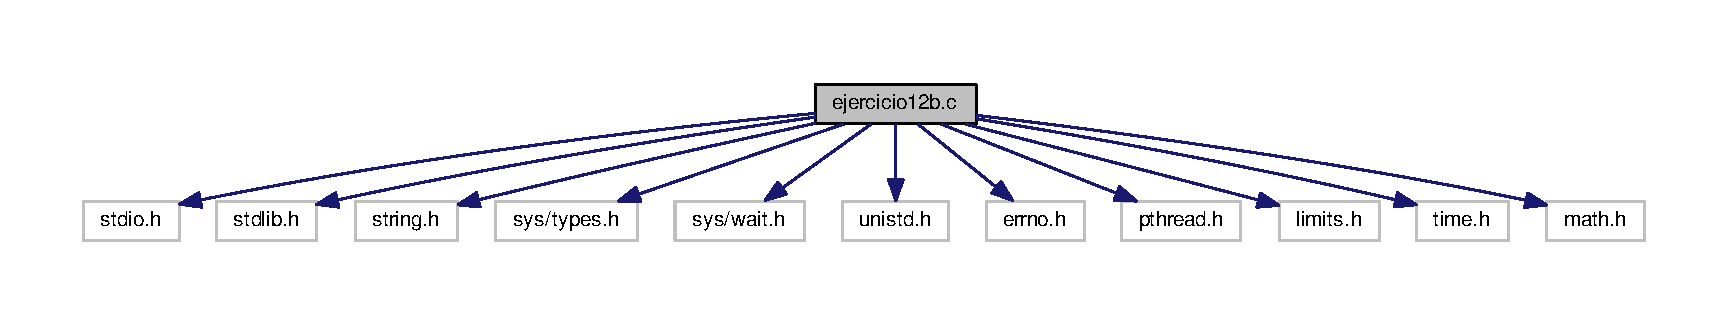
\includegraphics[width=350pt]{ejercicio12b_8c__incl}
\end{center}
\end{figure}
\subsection*{Classes}
\begin{DoxyCompactItemize}
\item 
struct \hyperlink{structStructure}{Structure}
\begin{DoxyCompactList}\small\item\em Estructura programa. \end{DoxyCompactList}\end{DoxyCompactItemize}
\subsection*{Macros}
\begin{DoxyCompactItemize}
\item 
\#define \hyperlink{ejercicio12b_8c_a05b49c662c073f89e86804f7856622a0}{L\+E\+N}~100
\item 
\#define \hyperlink{ejercicio12b_8c_a1dc0370947cd4d4485a36ad37de15139}{T\+E\+N\+T\+O\+T\+H\+E\+N\+I\+N\+E}~1000000000
\item 
\#define \hyperlink{ejercicio12b_8c_a469b1ab8d3ecbd62178c442e0d19c200}{N\+\_\+\+C\+H\+I\+L\+D\+S}~100
\end{DoxyCompactItemize}
\subsection*{Functions}
\begin{DoxyCompactItemize}
\item 
int \hyperlink{ejercicio12b_8c_ad6740255386952216cb75d813243a3ea}{is\+\_\+prime} (int n)
\begin{DoxyCompactList}\small\item\em evalua si un numero es primo o no. \end{DoxyCompactList}\item 
void $\ast$ \hyperlink{ejercicio12b_8c_a1996c5f0c98019293b7cfad2861f4547}{calculate\+\_\+primes} (void $\ast$arg)
\begin{DoxyCompactList}\small\item\em devuelve un array con los n\+\_\+primes primeros primos \end{DoxyCompactList}\item 
\hypertarget{ejercicio12b_8c_abf9e6b7e6f15df4b525a2e7705ba3089}{int {\bfseries main} (int argc, char const $\ast$argv\mbox{[}$\,$\mbox{]})}\label{ejercicio12b_8c_abf9e6b7e6f15df4b525a2e7705ba3089}

\end{DoxyCompactItemize}


\subsection{Detailed Description}
Ejercicio12b Creacion de 100 hilos y en cada uno se calculan los primeros N numeros primos, siendo N pasado como argumento entrada al programa. 

\begin{DoxyAuthor}{Author}
Alejandro Santorum \& David Cabornero 
\end{DoxyAuthor}
\begin{DoxyVersion}{Version}
1.\+0 
\end{DoxyVersion}
\begin{DoxyDate}{Date}
02-\/03-\/2018 
\end{DoxyDate}


\subsection{Macro Definition Documentation}
\hypertarget{ejercicio12b_8c_a05b49c662c073f89e86804f7856622a0}{\index{ejercicio12b.\+c@{ejercicio12b.\+c}!L\+E\+N@{L\+E\+N}}
\index{L\+E\+N@{L\+E\+N}!ejercicio12b.\+c@{ejercicio12b.\+c}}
\subsubsection[{L\+E\+N}]{\setlength{\rightskip}{0pt plus 5cm}\#define L\+E\+N~100}}\label{ejercicio12b_8c_a05b49c662c073f89e86804f7856622a0}
Longitud de las cadenas de caracteres \hypertarget{ejercicio12b_8c_a469b1ab8d3ecbd62178c442e0d19c200}{\index{ejercicio12b.\+c@{ejercicio12b.\+c}!N\+\_\+\+C\+H\+I\+L\+D\+S@{N\+\_\+\+C\+H\+I\+L\+D\+S}}
\index{N\+\_\+\+C\+H\+I\+L\+D\+S@{N\+\_\+\+C\+H\+I\+L\+D\+S}!ejercicio12b.\+c@{ejercicio12b.\+c}}
\subsubsection[{N\+\_\+\+C\+H\+I\+L\+D\+S}]{\setlength{\rightskip}{0pt plus 5cm}\#define N\+\_\+\+C\+H\+I\+L\+D\+S~100}}\label{ejercicio12b_8c_a469b1ab8d3ecbd62178c442e0d19c200}
Numero de procesos hijo \hypertarget{ejercicio12b_8c_a1dc0370947cd4d4485a36ad37de15139}{\index{ejercicio12b.\+c@{ejercicio12b.\+c}!T\+E\+N\+T\+O\+T\+H\+E\+N\+I\+N\+E@{T\+E\+N\+T\+O\+T\+H\+E\+N\+I\+N\+E}}
\index{T\+E\+N\+T\+O\+T\+H\+E\+N\+I\+N\+E@{T\+E\+N\+T\+O\+T\+H\+E\+N\+I\+N\+E}!ejercicio12b.\+c@{ejercicio12b.\+c}}
\subsubsection[{T\+E\+N\+T\+O\+T\+H\+E\+N\+I\+N\+E}]{\setlength{\rightskip}{0pt plus 5cm}\#define T\+E\+N\+T\+O\+T\+H\+E\+N\+I\+N\+E~1000000000}}\label{ejercicio12b_8c_a1dc0370947cd4d4485a36ad37de15139}
Constante 

\subsection{Function Documentation}
\hypertarget{ejercicio12b_8c_a1996c5f0c98019293b7cfad2861f4547}{\index{ejercicio12b.\+c@{ejercicio12b.\+c}!calculate\+\_\+primes@{calculate\+\_\+primes}}
\index{calculate\+\_\+primes@{calculate\+\_\+primes}!ejercicio12b.\+c@{ejercicio12b.\+c}}
\subsubsection[{calculate\+\_\+primes}]{\setlength{\rightskip}{0pt plus 5cm}void $\ast$ calculate\+\_\+primes (
\begin{DoxyParamCaption}
\item[{void $\ast$}]{arg}
\end{DoxyParamCaption}
)}}\label{ejercicio12b_8c_a1996c5f0c98019293b7cfad2861f4547}


devuelve un array con los n\+\_\+primes primeros primos 


\begin{DoxyParams}{Parameters}
{\em arg,estructura} & con todos los argumentos de la fuincion que queramos \\
\hline
\end{DoxyParams}
\begin{DoxyReturn}{Returns}
void$\ast$, debido a la utilizacion de hilos (threads) 
\end{DoxyReturn}
\hypertarget{ejercicio12b_8c_ad6740255386952216cb75d813243a3ea}{\index{ejercicio12b.\+c@{ejercicio12b.\+c}!is\+\_\+prime@{is\+\_\+prime}}
\index{is\+\_\+prime@{is\+\_\+prime}!ejercicio12b.\+c@{ejercicio12b.\+c}}
\subsubsection[{is\+\_\+prime}]{\setlength{\rightskip}{0pt plus 5cm}int is\+\_\+prime (
\begin{DoxyParamCaption}
\item[{int}]{n}
\end{DoxyParamCaption}
)}}\label{ejercicio12b_8c_ad6740255386952216cb75d813243a3ea}


evalua si un numero es primo o no. 


\begin{DoxyParams}{Parameters}
{\em n} & entero a ser evaluado \\
\hline
\end{DoxyParams}
\begin{DoxyReturn}{Returns}
true si es primo, false si no. 
\end{DoxyReturn}

\hypertarget{ejercicio13_8c}{\section{ejercicio13.\+c File Reference}
\label{ejercicio13_8c}\index{ejercicio13.\+c@{ejercicio13.\+c}}
}


Ejercicio13 Creacion de dos hilos. Cada uno multiplica una matriz por un escalar, imprimiendo el resultado cada vez que acaba de multiplicar una fila. Ademas, cada hilo sabe por donde va el otro.  


{\ttfamily \#include $<$stdio.\+h$>$}\\*
{\ttfamily \#include $<$stdlib.\+h$>$}\\*
{\ttfamily \#include $<$string.\+h$>$}\\*
{\ttfamily \#include $<$sys/types.\+h$>$}\\*
{\ttfamily \#include $<$sys/wait.\+h$>$}\\*
{\ttfamily \#include $<$unistd.\+h$>$}\\*
{\ttfamily \#include $<$errno.\+h$>$}\\*
{\ttfamily \#include $<$pthread.\+h$>$}\\*
{\ttfamily \#include $<$limits.\+h$>$}\\*
{\ttfamily \#include $<$time.\+h$>$}\\*
{\ttfamily \#include $<$math.\+h$>$}\\*
Include dependency graph for ejercicio13.\+c\+:
\nopagebreak
\begin{figure}[H]
\begin{center}
\leavevmode
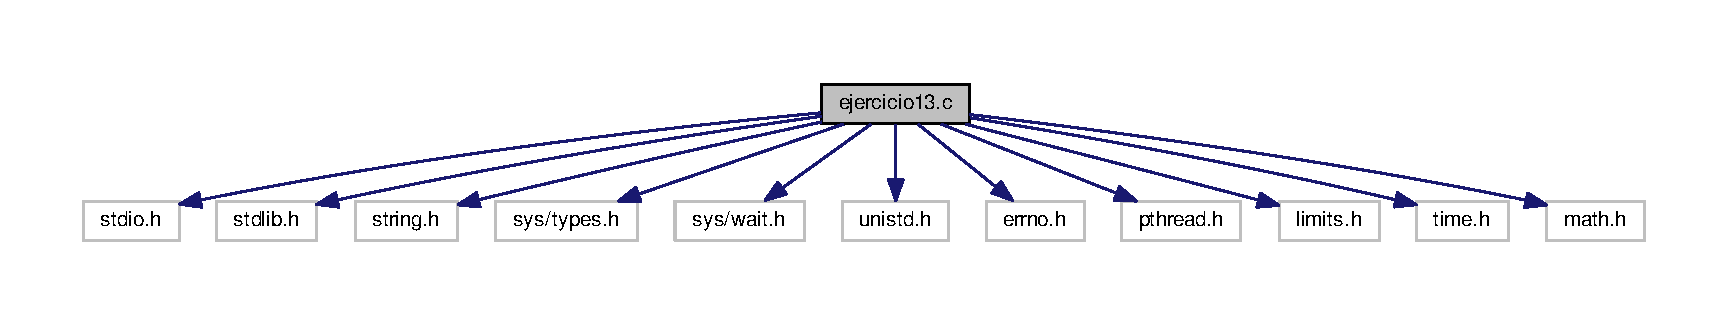
\includegraphics[width=350pt]{ejercicio13_8c__incl}
\end{center}
\end{figure}
\subsection*{Classes}
\begin{DoxyCompactItemize}
\item 
struct \hyperlink{structArgum}{Argum}
\begin{DoxyCompactList}\small\item\em Estructura de argumentos de entrada. \end{DoxyCompactList}\end{DoxyCompactItemize}
\subsection*{Macros}
\begin{DoxyCompactItemize}
\item 
\#define \hyperlink{ejercicio13_8c_a05b49c662c073f89e86804f7856622a0}{L\+E\+N}~50
\end{DoxyCompactItemize}
\subsection*{Functions}
\begin{DoxyCompactItemize}
\item 
void $\ast$ \hyperlink{ejercicio13_8c_a4dd6e3f428ac001b95d386b8045a2db9}{mult\+\_\+matrix} (void $\ast$arg)
\begin{DoxyCompactList}\small\item\em multiplica una matrix por un escalar. Ademas, indica el estado del hilo hermano. \end{DoxyCompactList}\item 
\hypertarget{ejercicio13_8c_abf9e6b7e6f15df4b525a2e7705ba3089}{int {\bfseries main} (int argc, char const $\ast$argv\mbox{[}$\,$\mbox{]})}\label{ejercicio13_8c_abf9e6b7e6f15df4b525a2e7705ba3089}

\end{DoxyCompactItemize}


\subsection{Detailed Description}
Ejercicio13 Creacion de dos hilos. Cada uno multiplica una matriz por un escalar, imprimiendo el resultado cada vez que acaba de multiplicar una fila. Ademas, cada hilo sabe por donde va el otro. 

\begin{DoxyAuthor}{Author}
Alejandro Santorum \& David Cabornero 
\end{DoxyAuthor}
\begin{DoxyVersion}{Version}
1.\+0 
\end{DoxyVersion}
\begin{DoxyDate}{Date}
02-\/03-\/2018 
\end{DoxyDate}


\subsection{Macro Definition Documentation}
\hypertarget{ejercicio13_8c_a05b49c662c073f89e86804f7856622a0}{\index{ejercicio13.\+c@{ejercicio13.\+c}!L\+E\+N@{L\+E\+N}}
\index{L\+E\+N@{L\+E\+N}!ejercicio13.\+c@{ejercicio13.\+c}}
\subsubsection[{L\+E\+N}]{\setlength{\rightskip}{0pt plus 5cm}\#define L\+E\+N~50}}\label{ejercicio13_8c_a05b49c662c073f89e86804f7856622a0}
Longitud cadena de caracteres 

\subsection{Function Documentation}
\hypertarget{ejercicio13_8c_a4dd6e3f428ac001b95d386b8045a2db9}{\index{ejercicio13.\+c@{ejercicio13.\+c}!mult\+\_\+matrix@{mult\+\_\+matrix}}
\index{mult\+\_\+matrix@{mult\+\_\+matrix}!ejercicio13.\+c@{ejercicio13.\+c}}
\subsubsection[{mult\+\_\+matrix}]{\setlength{\rightskip}{0pt plus 5cm}void $\ast$ mult\+\_\+matrix (
\begin{DoxyParamCaption}
\item[{void $\ast$}]{arg}
\end{DoxyParamCaption}
)}}\label{ejercicio13_8c_a4dd6e3f428ac001b95d386b8045a2db9}


multiplica una matrix por un escalar. Ademas, indica el estado del hilo hermano. 


\begin{DoxyParams}{Parameters}
{\em $\ast$arg} & estructura con todos los parametros necesarios \\
\hline
\end{DoxyParams}
\begin{DoxyReturn}{Returns}
void$\ast$, debido a politica de hilos 
\end{DoxyReturn}

\hypertarget{ejercicio4a_8c}{\section{ejercicio4a.\+c File Reference}
\label{ejercicio4a_8c}\index{ejercicio4a.\+c@{ejercicio4a.\+c}}
}


Ejercicio4a Modificación del código dado para que cada H\+I\+J\+O imprima su P\+I\+D y el P\+I\+D de su padre.  


{\ttfamily \#include $<$stdio.\+h$>$}\\*
{\ttfamily \#include $<$stdlib.\+h$>$}\\*
{\ttfamily \#include $<$sys/types.\+h$>$}\\*
{\ttfamily \#include $<$sys/wait.\+h$>$}\\*
{\ttfamily \#include $<$unistd.\+h$>$}\\*
Include dependency graph for ejercicio4a.\+c\+:
\nopagebreak
\begin{figure}[H]
\begin{center}
\leavevmode
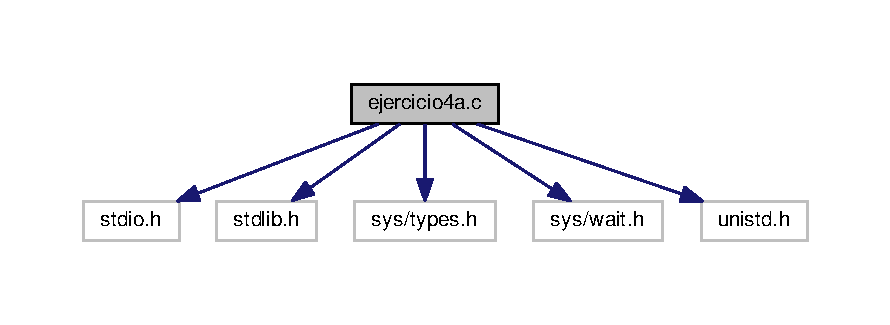
\includegraphics[width=350pt]{ejercicio4a_8c__incl}
\end{center}
\end{figure}
\subsection*{Macros}
\begin{DoxyCompactItemize}
\item 
\#define \hyperlink{ejercicio4a_8c_aea9978897a7765fbe7ece891bed80ee5}{P\+R\+O\+C\+\_\+\+N\+U\+M}~6
\end{DoxyCompactItemize}
\subsection*{Functions}
\begin{DoxyCompactItemize}
\item 
\hypertarget{ejercicio4a_8c_a840291bc02cba5474a4cb46a9b9566fe}{int {\bfseries main} (void)}\label{ejercicio4a_8c_a840291bc02cba5474a4cb46a9b9566fe}

\end{DoxyCompactItemize}


\subsection{Detailed Description}
Ejercicio4a Modificación del código dado para que cada H\+I\+J\+O imprima su P\+I\+D y el P\+I\+D de su padre. 

\begin{DoxyAuthor}{Author}
Alejandro Santorum \& David Cabornero 
\end{DoxyAuthor}
\begin{DoxyVersion}{Version}
1.\+0 
\end{DoxyVersion}
\begin{DoxyDate}{Date}
02-\/03-\/2018 
\end{DoxyDate}


\subsection{Macro Definition Documentation}
\hypertarget{ejercicio4a_8c_aea9978897a7765fbe7ece891bed80ee5}{\index{ejercicio4a.\+c@{ejercicio4a.\+c}!P\+R\+O\+C\+\_\+\+N\+U\+M@{P\+R\+O\+C\+\_\+\+N\+U\+M}}
\index{P\+R\+O\+C\+\_\+\+N\+U\+M@{P\+R\+O\+C\+\_\+\+N\+U\+M}!ejercicio4a.\+c@{ejercicio4a.\+c}}
\subsubsection[{P\+R\+O\+C\+\_\+\+N\+U\+M}]{\setlength{\rightskip}{0pt plus 5cm}\#define P\+R\+O\+C\+\_\+\+N\+U\+M~6}}\label{ejercicio4a_8c_aea9978897a7765fbe7ece891bed80ee5}
Número de procesos 
\hypertarget{ejercicio4b_8c}{\section{ejercicio4b.\+c File Reference}
\label{ejercicio4b_8c}\index{ejercicio4b.\+c@{ejercicio4b.\+c}}
}


Ejercicio4b Modificación del código dado para que cada H\+I\+J\+O imprima su P\+I\+D y el P\+I\+D de su padre. Se diferencia con el ejercicio anterior por la presencia de wait().  


{\ttfamily \#include $<$stdio.\+h$>$}\\*
{\ttfamily \#include $<$stdlib.\+h$>$}\\*
{\ttfamily \#include $<$sys/types.\+h$>$}\\*
{\ttfamily \#include $<$sys/wait.\+h$>$}\\*
{\ttfamily \#include $<$unistd.\+h$>$}\\*
Include dependency graph for ejercicio4b.\+c\+:
\nopagebreak
\begin{figure}[H]
\begin{center}
\leavevmode
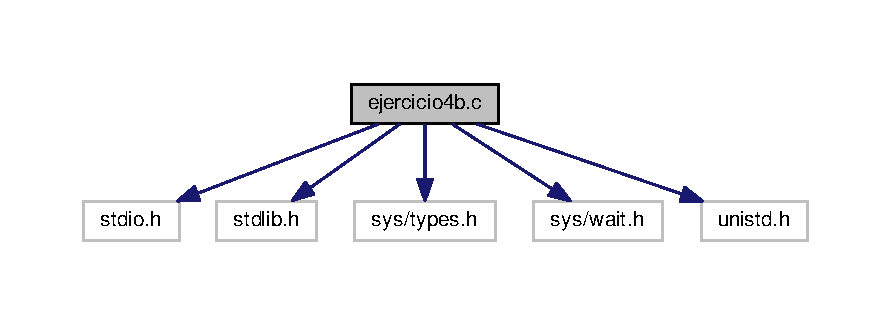
\includegraphics[width=350pt]{ejercicio4b_8c__incl}
\end{center}
\end{figure}
\subsection*{Macros}
\begin{DoxyCompactItemize}
\item 
\#define \hyperlink{ejercicio4b_8c_aea9978897a7765fbe7ece891bed80ee5}{P\+R\+O\+C\+\_\+\+N\+U\+M}~6
\end{DoxyCompactItemize}
\subsection*{Functions}
\begin{DoxyCompactItemize}
\item 
\hypertarget{ejercicio4b_8c_a840291bc02cba5474a4cb46a9b9566fe}{int {\bfseries main} (void)}\label{ejercicio4b_8c_a840291bc02cba5474a4cb46a9b9566fe}

\end{DoxyCompactItemize}


\subsection{Detailed Description}
Ejercicio4b Modificación del código dado para que cada H\+I\+J\+O imprima su P\+I\+D y el P\+I\+D de su padre. Se diferencia con el ejercicio anterior por la presencia de wait(). 

\begin{DoxyAuthor}{Author}
Alejandro Santorum \& David Cabornero 
\end{DoxyAuthor}
\begin{DoxyVersion}{Version}
1.\+0 
\end{DoxyVersion}
\begin{DoxyDate}{Date}
02-\/03-\/2018 
\end{DoxyDate}


\subsection{Macro Definition Documentation}
\hypertarget{ejercicio4b_8c_aea9978897a7765fbe7ece891bed80ee5}{\index{ejercicio4b.\+c@{ejercicio4b.\+c}!P\+R\+O\+C\+\_\+\+N\+U\+M@{P\+R\+O\+C\+\_\+\+N\+U\+M}}
\index{P\+R\+O\+C\+\_\+\+N\+U\+M@{P\+R\+O\+C\+\_\+\+N\+U\+M}!ejercicio4b.\+c@{ejercicio4b.\+c}}
\subsubsection[{P\+R\+O\+C\+\_\+\+N\+U\+M}]{\setlength{\rightskip}{0pt plus 5cm}\#define P\+R\+O\+C\+\_\+\+N\+U\+M~6}}\label{ejercicio4b_8c_aea9978897a7765fbe7ece891bed80ee5}
Número de procesos 
\hypertarget{ejercicio5a_8c}{\section{ejercicio5a.\+c File Reference}
\label{ejercicio5a_8c}\index{ejercicio5a.\+c@{ejercicio5a.\+c}}
}


Ejercicio5a Modificación del ejercicio4b para que cada proceso tengo un único hijo que sea esperado por su padre.  


{\ttfamily \#include $<$stdio.\+h$>$}\\*
{\ttfamily \#include $<$stdlib.\+h$>$}\\*
{\ttfamily \#include $<$sys/types.\+h$>$}\\*
{\ttfamily \#include $<$sys/wait.\+h$>$}\\*
{\ttfamily \#include $<$unistd.\+h$>$}\\*
Include dependency graph for ejercicio5a.\+c\+:
\nopagebreak
\begin{figure}[H]
\begin{center}
\leavevmode
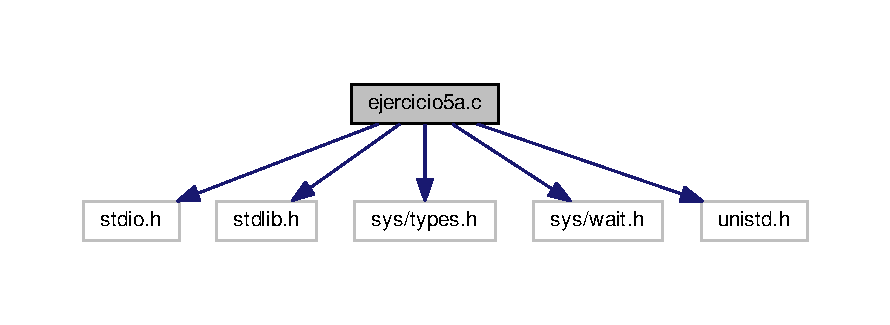
\includegraphics[width=350pt]{ejercicio5a_8c__incl}
\end{center}
\end{figure}
\subsection*{Macros}
\begin{DoxyCompactItemize}
\item 
\#define \hyperlink{ejercicio5a_8c_aea9978897a7765fbe7ece891bed80ee5}{P\+R\+O\+C\+\_\+\+N\+U\+M}~6
\end{DoxyCompactItemize}
\subsection*{Functions}
\begin{DoxyCompactItemize}
\item 
\hypertarget{ejercicio5a_8c_a840291bc02cba5474a4cb46a9b9566fe}{int {\bfseries main} (void)}\label{ejercicio5a_8c_a840291bc02cba5474a4cb46a9b9566fe}

\end{DoxyCompactItemize}


\subsection{Detailed Description}
Ejercicio5a Modificación del ejercicio4b para que cada proceso tengo un único hijo que sea esperado por su padre. 

\begin{DoxyAuthor}{Author}
Alejandro Santorum \& David Cabornero 
\end{DoxyAuthor}
\begin{DoxyVersion}{Version}
1.\+0 
\end{DoxyVersion}
\begin{DoxyDate}{Date}
02-\/03-\/2018 
\end{DoxyDate}


\subsection{Macro Definition Documentation}
\hypertarget{ejercicio5a_8c_aea9978897a7765fbe7ece891bed80ee5}{\index{ejercicio5a.\+c@{ejercicio5a.\+c}!P\+R\+O\+C\+\_\+\+N\+U\+M@{P\+R\+O\+C\+\_\+\+N\+U\+M}}
\index{P\+R\+O\+C\+\_\+\+N\+U\+M@{P\+R\+O\+C\+\_\+\+N\+U\+M}!ejercicio5a.\+c@{ejercicio5a.\+c}}
\subsubsection[{P\+R\+O\+C\+\_\+\+N\+U\+M}]{\setlength{\rightskip}{0pt plus 5cm}\#define P\+R\+O\+C\+\_\+\+N\+U\+M~6}}\label{ejercicio5a_8c_aea9978897a7765fbe7ece891bed80ee5}
Número de procesos 
\hypertarget{ejercicio5b_8c}{\section{ejercicio5b.\+c File Reference}
\label{ejercicio5b_8c}\index{ejercicio5b.\+c@{ejercicio5b.\+c}}
}


Ejercicio5b Modificación del ejercicio4b para que un proceso tenga un conjunto de hijos que serán esperados por el padre.  


{\ttfamily \#include $<$stdio.\+h$>$}\\*
{\ttfamily \#include $<$stdlib.\+h$>$}\\*
{\ttfamily \#include $<$sys/types.\+h$>$}\\*
{\ttfamily \#include $<$sys/wait.\+h$>$}\\*
{\ttfamily \#include $<$unistd.\+h$>$}\\*
Include dependency graph for ejercicio5b.\+c\+:
\nopagebreak
\begin{figure}[H]
\begin{center}
\leavevmode
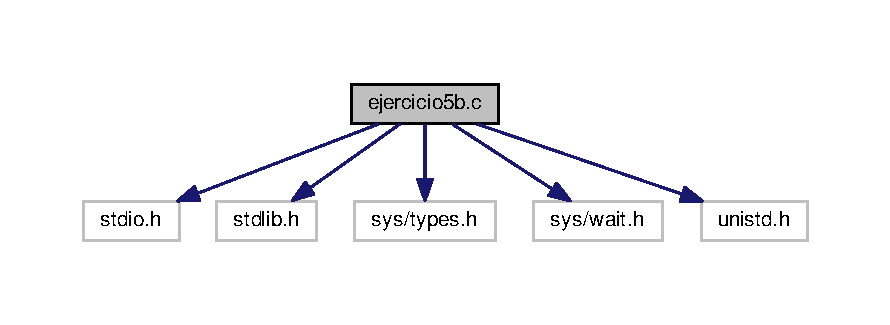
\includegraphics[width=350pt]{ejercicio5b_8c__incl}
\end{center}
\end{figure}
\subsection*{Macros}
\begin{DoxyCompactItemize}
\item 
\#define \hyperlink{ejercicio5b_8c_aea9978897a7765fbe7ece891bed80ee5}{P\+R\+O\+C\+\_\+\+N\+U\+M}~6
\end{DoxyCompactItemize}
\subsection*{Functions}
\begin{DoxyCompactItemize}
\item 
\hypertarget{ejercicio5b_8c_a840291bc02cba5474a4cb46a9b9566fe}{int {\bfseries main} (void)}\label{ejercicio5b_8c_a840291bc02cba5474a4cb46a9b9566fe}

\end{DoxyCompactItemize}


\subsection{Detailed Description}
Ejercicio5b Modificación del ejercicio4b para que un proceso tenga un conjunto de hijos que serán esperados por el padre. 

\begin{DoxyAuthor}{Author}
Alejandro Santorum \& David Cabornero 
\end{DoxyAuthor}
\begin{DoxyVersion}{Version}
1.\+0 
\end{DoxyVersion}
\begin{DoxyDate}{Date}
02-\/03-\/2018 
\end{DoxyDate}


\subsection{Macro Definition Documentation}
\hypertarget{ejercicio5b_8c_aea9978897a7765fbe7ece891bed80ee5}{\index{ejercicio5b.\+c@{ejercicio5b.\+c}!P\+R\+O\+C\+\_\+\+N\+U\+M@{P\+R\+O\+C\+\_\+\+N\+U\+M}}
\index{P\+R\+O\+C\+\_\+\+N\+U\+M@{P\+R\+O\+C\+\_\+\+N\+U\+M}!ejercicio5b.\+c@{ejercicio5b.\+c}}
\subsubsection[{P\+R\+O\+C\+\_\+\+N\+U\+M}]{\setlength{\rightskip}{0pt plus 5cm}\#define P\+R\+O\+C\+\_\+\+N\+U\+M~6}}\label{ejercicio5b_8c_aea9978897a7765fbe7ece891bed80ee5}
Número de procesos 
\hypertarget{ejercicio6_8c}{\section{ejercicio6.\+c File Reference}
\label{ejercicio6_8c}\index{ejercicio6.\+c@{ejercicio6.\+c}}
}


Ejercicio6 Comprobación de si dos procesos (padre e hijo) comparten la misma zona de memoria una vez lanzados.  


{\ttfamily \#include $<$stdio.\+h$>$}\\*
{\ttfamily \#include $<$stdlib.\+h$>$}\\*
{\ttfamily \#include $<$string.\+h$>$}\\*
{\ttfamily \#include $<$sys/types.\+h$>$}\\*
{\ttfamily \#include $<$sys/wait.\+h$>$}\\*
{\ttfamily \#include $<$unistd.\+h$>$}\\*
{\ttfamily \#include $<$errno.\+h$>$}\\*
Include dependency graph for ejercicio6.\+c\+:
\nopagebreak
\begin{figure}[H]
\begin{center}
\leavevmode
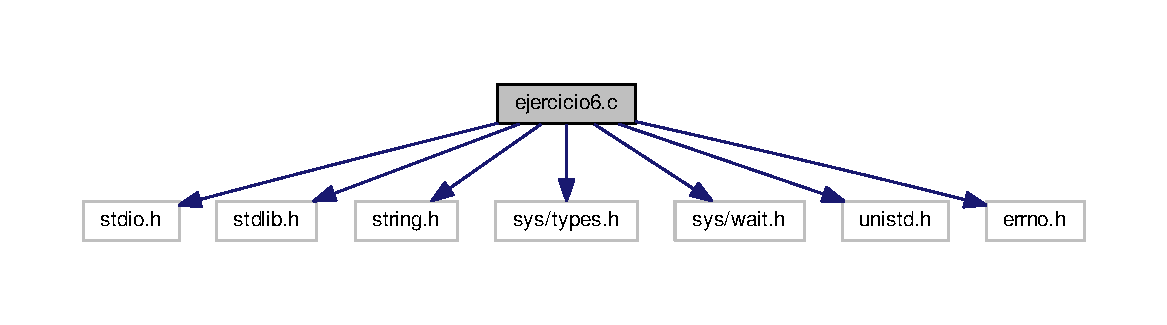
\includegraphics[width=350pt]{ejercicio6_8c__incl}
\end{center}
\end{figure}
\subsection*{Classes}
\begin{DoxyCompactItemize}
\item 
struct \hyperlink{structStructure}{Structure}
\begin{DoxyCompactList}\small\item\em Estructura programa. \end{DoxyCompactList}\end{DoxyCompactItemize}
\subsection*{Macros}
\begin{DoxyCompactItemize}
\item 
\#define \hyperlink{ejercicio6_8c_a05b49c662c073f89e86804f7856622a0}{L\+E\+N}~80
\end{DoxyCompactItemize}
\subsection*{Functions}
\begin{DoxyCompactItemize}
\item 
\hypertarget{ejercicio6_8c_ae66f6b31b5ad750f1fe042a706a4e3d4}{int {\bfseries main} ()}\label{ejercicio6_8c_ae66f6b31b5ad750f1fe042a706a4e3d4}

\end{DoxyCompactItemize}


\subsection{Detailed Description}
Ejercicio6 Comprobación de si dos procesos (padre e hijo) comparten la misma zona de memoria una vez lanzados. 

\begin{DoxyAuthor}{Author}
Alejandro Santorum \& David Cabornero (G2202) 
\end{DoxyAuthor}
\begin{DoxyVersion}{Version}
1.\+0 
\end{DoxyVersion}
\begin{DoxyDate}{Date}
02-\/03-\/2018 
\end{DoxyDate}


\subsection{Macro Definition Documentation}
\hypertarget{ejercicio6_8c_a05b49c662c073f89e86804f7856622a0}{\index{ejercicio6.\+c@{ejercicio6.\+c}!L\+E\+N@{L\+E\+N}}
\index{L\+E\+N@{L\+E\+N}!ejercicio6.\+c@{ejercicio6.\+c}}
\subsubsection[{L\+E\+N}]{\setlength{\rightskip}{0pt plus 5cm}\#define L\+E\+N~80}}\label{ejercicio6_8c_a05b49c662c073f89e86804f7856622a0}
Longitud cadena de caracteres 
\hypertarget{ejercicio8__1_8c}{\section{ejercicio8\+\_\+1.\+c File Reference}
\label{ejercicio8__1_8c}\index{ejercicio8\+\_\+1.\+c@{ejercicio8\+\_\+1.\+c}}
}


Ejercicio8\+\_\+1 Ejecución de varios programas desde el primero pasado como argumento de entrada hasta el ultimo.  


{\ttfamily \#include $<$stdio.\+h$>$}\\*
{\ttfamily \#include $<$stdlib.\+h$>$}\\*
{\ttfamily \#include $<$string.\+h$>$}\\*
{\ttfamily \#include $<$sys/types.\+h$>$}\\*
{\ttfamily \#include $<$sys/wait.\+h$>$}\\*
{\ttfamily \#include $<$unistd.\+h$>$}\\*
{\ttfamily \#include $<$errno.\+h$>$}\\*
Include dependency graph for ejercicio8\+\_\+1.\+c\+:
\nopagebreak
\begin{figure}[H]
\begin{center}
\leavevmode
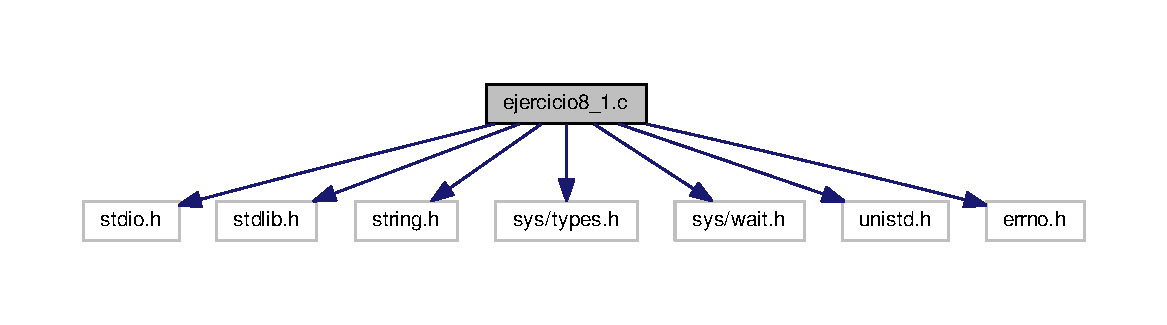
\includegraphics[width=350pt]{ejercicio8__1_8c__incl}
\end{center}
\end{figure}
\subsection*{Macros}
\begin{DoxyCompactItemize}
\item 
\#define \hyperlink{ejercicio8__1_8c_a943afdb7a415a72b444ecbc5c9286fae}{P\+A\+T\+H\+\_\+\+L\+E\+N}~100
\end{DoxyCompactItemize}
\subsection*{Functions}
\begin{DoxyCompactItemize}
\item 
\hypertarget{ejercicio8__1_8c_a3c04138a5bfe5d72780bb7e82a18e627}{int {\bfseries main} (int argc, char $\ast$$\ast$argv)}\label{ejercicio8__1_8c_a3c04138a5bfe5d72780bb7e82a18e627}

\end{DoxyCompactItemize}


\subsection{Detailed Description}
Ejercicio8\+\_\+1 Ejecución de varios programas desde el primero pasado como argumento de entrada hasta el ultimo. 

\begin{DoxyAuthor}{Author}
Alejandro Santorum \& David Cabornero (G2202) 
\end{DoxyAuthor}
\begin{DoxyVersion}{Version}
1.\+0 
\end{DoxyVersion}
\begin{DoxyDate}{Date}
02-\/03-\/2018 
\end{DoxyDate}


\subsection{Macro Definition Documentation}
\hypertarget{ejercicio8__1_8c_a943afdb7a415a72b444ecbc5c9286fae}{\index{ejercicio8\+\_\+1.\+c@{ejercicio8\+\_\+1.\+c}!P\+A\+T\+H\+\_\+\+L\+E\+N@{P\+A\+T\+H\+\_\+\+L\+E\+N}}
\index{P\+A\+T\+H\+\_\+\+L\+E\+N@{P\+A\+T\+H\+\_\+\+L\+E\+N}!ejercicio8\+\_\+1.\+c@{ejercicio8\+\_\+1.\+c}}
\subsubsection[{P\+A\+T\+H\+\_\+\+L\+E\+N}]{\setlength{\rightskip}{0pt plus 5cm}\#define P\+A\+T\+H\+\_\+\+L\+E\+N~100}}\label{ejercicio8__1_8c_a943afdb7a415a72b444ecbc5c9286fae}
Longitud cadenas de caracteres 
\hypertarget{ejercicio8__2_8c}{\section{ejercicio8\+\_\+2.\+c File Reference}
\label{ejercicio8__2_8c}\index{ejercicio8\+\_\+2.\+c@{ejercicio8\+\_\+2.\+c}}
}


Ejercicio8\+\_\+2 Ejecución de varios programas desde el ultimo pasado como argumento de entrada hasta el primero.  


{\ttfamily \#include $<$stdio.\+h$>$}\\*
{\ttfamily \#include $<$stdlib.\+h$>$}\\*
{\ttfamily \#include $<$string.\+h$>$}\\*
{\ttfamily \#include $<$sys/types.\+h$>$}\\*
{\ttfamily \#include $<$sys/wait.\+h$>$}\\*
{\ttfamily \#include $<$unistd.\+h$>$}\\*
{\ttfamily \#include $<$errno.\+h$>$}\\*
Include dependency graph for ejercicio8\+\_\+2.\+c\+:
\nopagebreak
\begin{figure}[H]
\begin{center}
\leavevmode
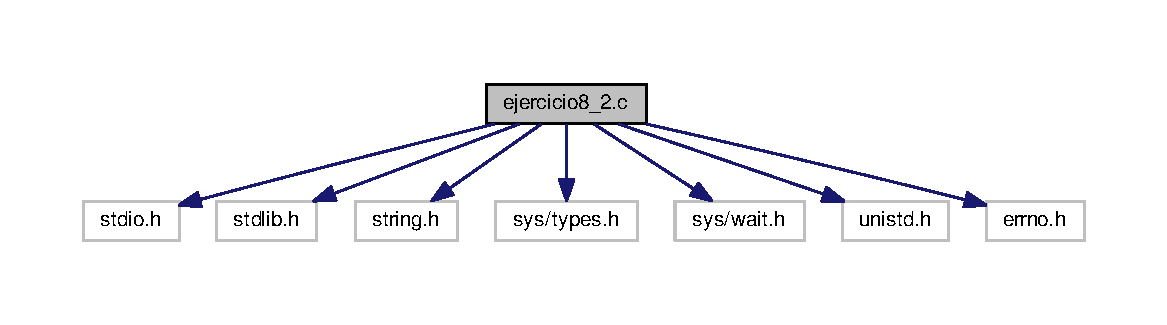
\includegraphics[width=350pt]{ejercicio8__2_8c__incl}
\end{center}
\end{figure}
\subsection*{Macros}
\begin{DoxyCompactItemize}
\item 
\#define \hyperlink{ejercicio8__2_8c_a943afdb7a415a72b444ecbc5c9286fae}{P\+A\+T\+H\+\_\+\+L\+E\+N}~100
\end{DoxyCompactItemize}
\subsection*{Functions}
\begin{DoxyCompactItemize}
\item 
\hypertarget{ejercicio8__2_8c_a3c04138a5bfe5d72780bb7e82a18e627}{int {\bfseries main} (int argc, char $\ast$$\ast$argv)}\label{ejercicio8__2_8c_a3c04138a5bfe5d72780bb7e82a18e627}

\end{DoxyCompactItemize}


\subsection{Detailed Description}
Ejercicio8\+\_\+2 Ejecución de varios programas desde el ultimo pasado como argumento de entrada hasta el primero. 

\begin{DoxyAuthor}{Author}
Alejandro Santorum \& David Cabornero (G2202) 
\end{DoxyAuthor}
\begin{DoxyVersion}{Version}
1.\+0 
\end{DoxyVersion}
\begin{DoxyDate}{Date}
02-\/03-\/2018 
\end{DoxyDate}


\subsection{Macro Definition Documentation}
\hypertarget{ejercicio8__2_8c_a943afdb7a415a72b444ecbc5c9286fae}{\index{ejercicio8\+\_\+2.\+c@{ejercicio8\+\_\+2.\+c}!P\+A\+T\+H\+\_\+\+L\+E\+N@{P\+A\+T\+H\+\_\+\+L\+E\+N}}
\index{P\+A\+T\+H\+\_\+\+L\+E\+N@{P\+A\+T\+H\+\_\+\+L\+E\+N}!ejercicio8\+\_\+2.\+c@{ejercicio8\+\_\+2.\+c}}
\subsubsection[{P\+A\+T\+H\+\_\+\+L\+E\+N}]{\setlength{\rightskip}{0pt plus 5cm}\#define P\+A\+T\+H\+\_\+\+L\+E\+N~100}}\label{ejercicio8__2_8c_a943afdb7a415a72b444ecbc5c9286fae}
Longitud cadenas de caracteres 
\hypertarget{ejercicio9_8c}{\section{ejercicio9.\+c File Reference}
\label{ejercicio9_8c}\index{ejercicio9.\+c@{ejercicio9.\+c}}
}


Ejercicio9 Ejercicio de comunicación bidireccional entre procesos utilizando tuberias (pipes)  


{\ttfamily \#include $<$stdio.\+h$>$}\\*
{\ttfamily \#include $<$stdlib.\+h$>$}\\*
{\ttfamily \#include $<$string.\+h$>$}\\*
{\ttfamily \#include $<$math.\+h$>$}\\*
{\ttfamily \#include $<$sys/types.\+h$>$}\\*
{\ttfamily \#include $<$sys/wait.\+h$>$}\\*
{\ttfamily \#include $<$unistd.\+h$>$}\\*
{\ttfamily \#include $<$errno.\+h$>$}\\*
Include dependency graph for ejercicio9.\+c\+:
\nopagebreak
\begin{figure}[H]
\begin{center}
\leavevmode
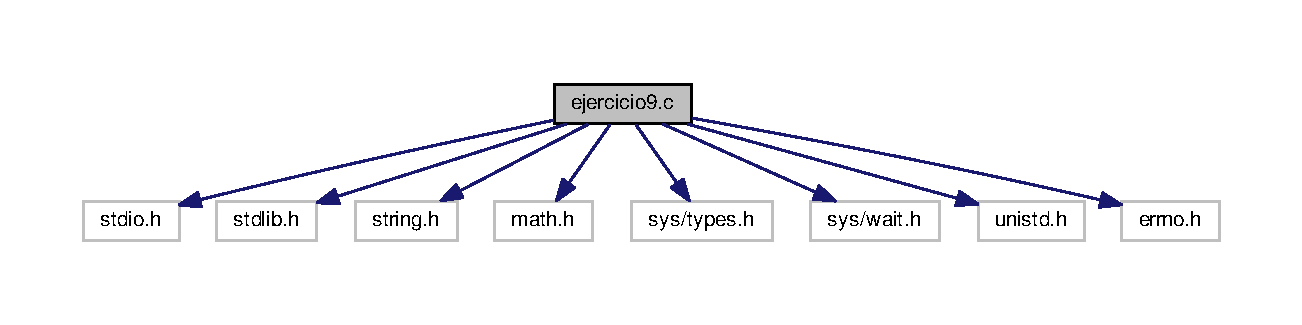
\includegraphics[width=350pt]{ejercicio9_8c__incl}
\end{center}
\end{figure}
\subsection*{Macros}
\begin{DoxyCompactItemize}
\item 
\#define \hyperlink{ejercicio9_8c_ada74e7db007a68e763f20c17f2985356}{R\+E\+A\+D}~0
\item 
\#define \hyperlink{ejercicio9_8c_aa10f470e996d0f51210d24f442d25e1e}{W\+R\+I\+T\+E}~1
\item 
\#define \hyperlink{ejercicio9_8c_a469b1ab8d3ecbd62178c442e0d19c200}{N\+\_\+\+C\+H\+I\+L\+D\+S}~4
\item 
\#define \hyperlink{ejercicio9_8c_a05b49c662c073f89e86804f7856622a0}{L\+E\+N}~300
\end{DoxyCompactItemize}
\subsection*{Functions}
\begin{DoxyCompactItemize}
\item 
int \hyperlink{ejercicio9_8c_a4aa006d6fead344c31cadac2d1292a8e}{split\+\_\+first} (char $\ast$str)
\begin{DoxyCompactList}\small\item\em separa de una cadena el primero Operando \end{DoxyCompactList}\item 
int \hyperlink{ejercicio9_8c_a6b950f9c2c30c4e1c810b97ee01f141b}{split\+\_\+second} (char $\ast$str)
\begin{DoxyCompactList}\small\item\em separa de una cadena el segundo Operando \end{DoxyCompactList}\item 
long long \hyperlink{ejercicio9_8c_a08c1504776e3d3a7294db624ce6d19f5}{factorial} (int a)
\begin{DoxyCompactList}\small\item\em calcula el factorial \end{DoxyCompactList}\item 
int \hyperlink{ejercicio9_8c_aa80441bd92270f050b0796561243f410}{abs} (int a)
\begin{DoxyCompactList}\small\item\em calcula el valor absoluto \end{DoxyCompactList}\item 
\hypertarget{ejercicio9_8c_ae66f6b31b5ad750f1fe042a706a4e3d4}{int {\bfseries main} ()}\label{ejercicio9_8c_ae66f6b31b5ad750f1fe042a706a4e3d4}

\end{DoxyCompactItemize}


\subsection{Detailed Description}
Ejercicio9 Ejercicio de comunicación bidireccional entre procesos utilizando tuberias (pipes) 

\begin{DoxyAuthor}{Author}
Alejandro Santorum \& David Cabornero (G2202) 
\end{DoxyAuthor}
\begin{DoxyVersion}{Version}
1.\+0 
\end{DoxyVersion}
\begin{DoxyDate}{Date}
02-\/03-\/2018 
\end{DoxyDate}


\subsection{Macro Definition Documentation}
\hypertarget{ejercicio9_8c_a05b49c662c073f89e86804f7856622a0}{\index{ejercicio9.\+c@{ejercicio9.\+c}!L\+E\+N@{L\+E\+N}}
\index{L\+E\+N@{L\+E\+N}!ejercicio9.\+c@{ejercicio9.\+c}}
\subsubsection[{L\+E\+N}]{\setlength{\rightskip}{0pt plus 5cm}\#define L\+E\+N~300}}\label{ejercicio9_8c_a05b49c662c073f89e86804f7856622a0}
Longitud de las cadenas de caracteres \hypertarget{ejercicio9_8c_a469b1ab8d3ecbd62178c442e0d19c200}{\index{ejercicio9.\+c@{ejercicio9.\+c}!N\+\_\+\+C\+H\+I\+L\+D\+S@{N\+\_\+\+C\+H\+I\+L\+D\+S}}
\index{N\+\_\+\+C\+H\+I\+L\+D\+S@{N\+\_\+\+C\+H\+I\+L\+D\+S}!ejercicio9.\+c@{ejercicio9.\+c}}
\subsubsection[{N\+\_\+\+C\+H\+I\+L\+D\+S}]{\setlength{\rightskip}{0pt plus 5cm}\#define N\+\_\+\+C\+H\+I\+L\+D\+S~4}}\label{ejercicio9_8c_a469b1ab8d3ecbd62178c442e0d19c200}
Numero de procesos hijo \hypertarget{ejercicio9_8c_ada74e7db007a68e763f20c17f2985356}{\index{ejercicio9.\+c@{ejercicio9.\+c}!R\+E\+A\+D@{R\+E\+A\+D}}
\index{R\+E\+A\+D@{R\+E\+A\+D}!ejercicio9.\+c@{ejercicio9.\+c}}
\subsubsection[{R\+E\+A\+D}]{\setlength{\rightskip}{0pt plus 5cm}\#define R\+E\+A\+D~0}}\label{ejercicio9_8c_ada74e7db007a68e763f20c17f2985356}
Macro para lectura en tuberias \hypertarget{ejercicio9_8c_aa10f470e996d0f51210d24f442d25e1e}{\index{ejercicio9.\+c@{ejercicio9.\+c}!W\+R\+I\+T\+E@{W\+R\+I\+T\+E}}
\index{W\+R\+I\+T\+E@{W\+R\+I\+T\+E}!ejercicio9.\+c@{ejercicio9.\+c}}
\subsubsection[{W\+R\+I\+T\+E}]{\setlength{\rightskip}{0pt plus 5cm}\#define W\+R\+I\+T\+E~1}}\label{ejercicio9_8c_aa10f470e996d0f51210d24f442d25e1e}
Macro para escritura en tuberias 

\subsection{Function Documentation}
\hypertarget{ejercicio9_8c_aa80441bd92270f050b0796561243f410}{\index{ejercicio9.\+c@{ejercicio9.\+c}!abs@{abs}}
\index{abs@{abs}!ejercicio9.\+c@{ejercicio9.\+c}}
\subsubsection[{abs}]{\setlength{\rightskip}{0pt plus 5cm}int abs (
\begin{DoxyParamCaption}
\item[{int}]{a}
\end{DoxyParamCaption}
)}}\label{ejercicio9_8c_aa80441bd92270f050b0796561243f410}


calcula el valor absoluto 


\begin{DoxyParams}{Parameters}
{\em a} & entero para calcular su valor absoluto \\
\hline
\end{DoxyParams}
\begin{DoxyReturn}{Returns}
entero valor absoluto 
\end{DoxyReturn}
\hypertarget{ejercicio9_8c_a08c1504776e3d3a7294db624ce6d19f5}{\index{ejercicio9.\+c@{ejercicio9.\+c}!factorial@{factorial}}
\index{factorial@{factorial}!ejercicio9.\+c@{ejercicio9.\+c}}
\subsubsection[{factorial}]{\setlength{\rightskip}{0pt plus 5cm}long long factorial (
\begin{DoxyParamCaption}
\item[{int}]{a}
\end{DoxyParamCaption}
)}}\label{ejercicio9_8c_a08c1504776e3d3a7294db624ce6d19f5}


calcula el factorial 


\begin{DoxyParams}{Parameters}
{\em a} & entero para calcular su factorial \\
\hline
\end{DoxyParams}
\begin{DoxyReturn}{Returns}
entero factorial 
\end{DoxyReturn}
\hypertarget{ejercicio9_8c_a4aa006d6fead344c31cadac2d1292a8e}{\index{ejercicio9.\+c@{ejercicio9.\+c}!split\+\_\+first@{split\+\_\+first}}
\index{split\+\_\+first@{split\+\_\+first}!ejercicio9.\+c@{ejercicio9.\+c}}
\subsubsection[{split\+\_\+first}]{\setlength{\rightskip}{0pt plus 5cm}int split\+\_\+first (
\begin{DoxyParamCaption}
\item[{char $\ast$}]{str}
\end{DoxyParamCaption}
)}}\label{ejercicio9_8c_a4aa006d6fead344c31cadac2d1292a8e}


separa de una cadena el primero Operando 


\begin{DoxyParams}{Parameters}
{\em str} & cadena para ser separada \\
\hline
\end{DoxyParams}
\begin{DoxyReturn}{Returns}
entero que es el primer operando 
\end{DoxyReturn}
\hypertarget{ejercicio9_8c_a6b950f9c2c30c4e1c810b97ee01f141b}{\index{ejercicio9.\+c@{ejercicio9.\+c}!split\+\_\+second@{split\+\_\+second}}
\index{split\+\_\+second@{split\+\_\+second}!ejercicio9.\+c@{ejercicio9.\+c}}
\subsubsection[{split\+\_\+second}]{\setlength{\rightskip}{0pt plus 5cm}int split\+\_\+second (
\begin{DoxyParamCaption}
\item[{char $\ast$}]{str}
\end{DoxyParamCaption}
)}}\label{ejercicio9_8c_a6b950f9c2c30c4e1c810b97ee01f141b}


separa de una cadena el segundo Operando 


\begin{DoxyParams}{Parameters}
{\em str} & cadena para ser separada \\
\hline
\end{DoxyParams}
\begin{DoxyReturn}{Returns}
entero que es el segundo operando 
\end{DoxyReturn}

%--- End generated contents ---

% Index
\newpage
\phantomsection
\addcontentsline{toc}{chapter}{Index}
\printindex

\end{document}
